\documentclass[a4paper, 12pt]{article}

\usepackage[T2A]{fontenc}
\usepackage[utf8]{inputenc}
\usepackage[english,russian]{babel}
\usepackage{amsmath, amsfonts, amssymb, amsthm, mathtools}

\usepackage{indentfirst}
\usepackage{icomma}
\usepackage{hyperref}
\usepackage{soulutf8}

\usepackage{multirow}
\usepackage{hhline}
\usepackage{graphicx}

\usepackage{tikz}
\usetikzlibrary{calc}

\usepackage{diagbox}
\usepackage{wrapfig}
\usepackage{caption}
\usepackage{subcaption}

\usepackage{geometry}
\geometry{top=25mm}
\geometry{bottom=30mm}
\geometry{left=20mm}
\geometry{right=20mm}

\renewcommand{\epsilon}{\varepsilon}
\renewcommand{\phi}{\varphi}
\newcommand{\mean}[1]{\left<#1\right>}

\title{\textbf{Работа 1.4.1}\linebreak Изучение физического маятника}
\author{Константин Ерёмин Б03-204}
\date{Ноябрь 2022}

\begin{document}
    \maketitle

    \section{Введение}
        \begin{target}
            исследовать зависимость периода колебаний физического маятника от его момента инерции.
        \end{target}

        \begin{setting}
            физический маятник в виде однородного стержня, опорная призма, математический маятник, счётчик числа колебаний, линейка, секундомер.
        \end{setting}

    \section{Теоретическое описание работы}
        \begin{wrapfigure}{h!}{0.3\textwidth}
            \vspace{-0.5cm}
            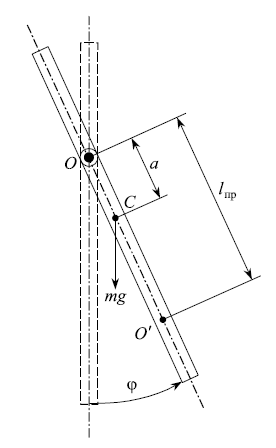
\includegraphics[width=0.25\textwidth]{pendulum}
            \caption{Физический маятник}
            \label{fig:pendulum}
        \end{wrapfigure}

        Физическим маятником называют твёрдое тело, которое под действием силы тяжести может свободно качаться вокруг неподвижной горизонтальной оси. Его движение описывается уравнением
        \begin{equation}
            I\frac{d^2\phi}{dt^2}=M,
        \end{equation}
        где $I$ "--- момент инерции маятника, $\phi$ "--- угол отклонения маятника от положения равновесия, $t$ "--- время, $M$ "--- момент сил, действующих на маятник.

        В данной работе в качестве физического маятника (\ref{fig:pendulum}) используется стальной стержень длиной $l$. На призме закрепляется опорная призма, ребро которой является осью качания маятника. Призму можно перремещать вдоль стержня, меняя таким образом расстояние $OC$ от точки опоры маятника до его центра масс. Пусть это расстояние равно $a$. Тогда по теореме Гюйгенса-Штейнера момент инерции маятника равен
        \begin{equation}
            I = \frac{ml^2}{12} + ma^2,
        \end{equation}
        где $m$ "--- масса маятника.

        Период колебаний \emph{физического} маятника определяется формулой
        \begin{equation}
            \label{eq:period}
            T = \frac{2\pi}{\omega} = 2\pi\sqrt{\frac{a^2+\frac{l^2}{12}}{ag}}.
        \end{equation}

        Период колебаний \emph{математического} маятника определяется формулой
        \begin{equation}
            T' = \frac{2\pi}{\omega'} = 2\pi\sqrt{\frac{l'}{g}},
        \end{equation}
        где $l'$ "--- длина математического маятника. Поэтому величину
        \begin{equation}
            l_\text{пр} = a + \frac{l^2}{12a}
            \label{eq:length}
        \end{equation}
        называют приведённой длиной физического маятника. Точку $O'$, отстоящую от точки опоры $O$ на расстояние $l_\text{пр}$, называют центром качания физического маятника. Точка опоры и центр качания обратимы, т.е. при качании вокруг точки $O'$ период будем таким же, как и при качании вокруг точки $O$.
        Справедливость этого утверждения проверяется в настоящей работе, также проверяется формула \refeq{eq:period}. В качестве математического маятника используется маленький свинцовый шарик, длину подвеса которого можно изменять.

    \section{Ход работы}
        \subsection{Подбор амплитуды}    
            Найдём период колебаний по продолжительности одной сотни колебаний при различных начальных отклонениях $\phi_0$, что отражено в таблице. Учтём ошибки измерения: абсолютная погрешность измерения времени человеком составляет $0.3$ секунды (время реакции), погрешнось секундомера --- $0.1$ секунды. Таким образом, при отсчёте сотни колебаний ошибки уменьшатся в \emph{сто} раз и полная погрешность составит
            \[\sigma_T = \sqrt{\left(\frac{0.3}{100}\right)^2 + \left(\frac{0.1}{100}\right)^2} \approx 0.003\text{ c}\].

            \begin{table}[h]
                \centering
                \begin{tabular}{|c|c|c|c|}
                    \hline
                    $\phi_0, ^\circ$ & 10 & 6 & 2.5 \\
                    \hline
                    $\tau\text{, с}$ & 161.0 & 160.8 & 162.4 \\
                    \hline
                    $T\text{, c}$ & 1.610 & 1.608 & 1.624 \\
                    \hline
                \end{tabular}
                \caption{Измерение периодов колебаний при различных углах отклонения}
                \label{table:angles}   
            \end{table}

            При непосредственной экспериментальной работе период будет измеряться по времени \emph{20} колебаний, и в таком случае погрешность составляет \underline{$\sigma_T \approx 0.016\text{ с}$}, поэтому в эсперименте можно использовать начальные отклонения в диапазоне $2.5$--$10^\circ$, так как в пределах данной погрешности периоды колебаний совпадают.

        \subsection{Проведение серии измерений}
            \begin{table}
                \centering
                \begin{tabular}{|c|c|c|c|c|c|c|c|c|c|c|}
                    \hline
                    a, м & 0.46 & 0.44 & 0.4 & 0.38 & 0.34 & 0.3 & 0.25 & 0.18 & 0.12 & 0.06 \\
                    \hline
                    t, с & 32.2 & 31.9 & 31.32 & 31.16 & 30.81 & 30.5 & 30.55 & 31.9 & 35.45 & 45.27 \\
                    \hline
                    T, с & 1.61 & 1.60 & 1.57 & 1.56 & 1.54 & 1.53 & 1.53 & 1.56 & 1.77 & 2.26 \\
                    \hline
                \end{tabular}
                \caption{Измерения периодов колебаний}
                \label{table:periods}
            \end{table}

            Исследуем зависимость периода колебаний $T$ от расстояния $a$ между точкой опоры и центром масс: будем измерять $T$ при различных $a$, занося результаты в таблицу \ref{table:periods}. Построим график $T(a)$ (рисунок \ref{fig:direct}). Как и ожидалось, зависимость $T(a)$ не является линейной. Преобразуем формулу \ref{eq:period} и построим линейный график $T^2a\left(a^2\right)$ (рис. \ref{fig:linear}):
            \begin{equation}
                T^2a = \frac{4\pi^2}{g}a^2 + \frac{4\pi^2}{g}\frac{l^2}{12}
            \end{equation}

            \begin{figure}
                \centering
                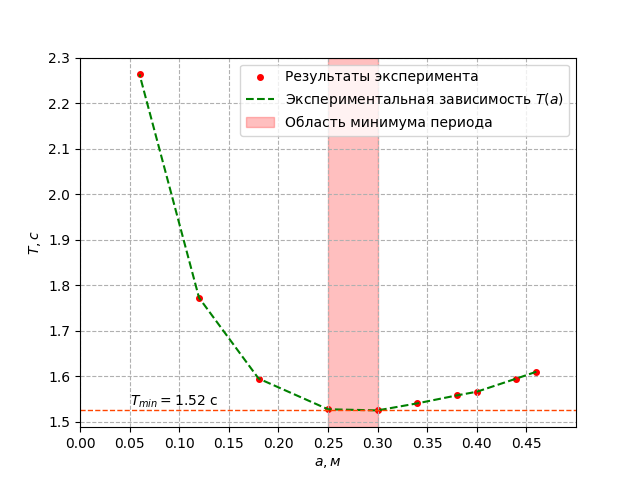
\includegraphics[width=0.75\linewidth]{direct.png}
                \caption{График $T(a)$}
                \label{fig:direct}
            \end{figure}
            \begin{figure}
                \centering
                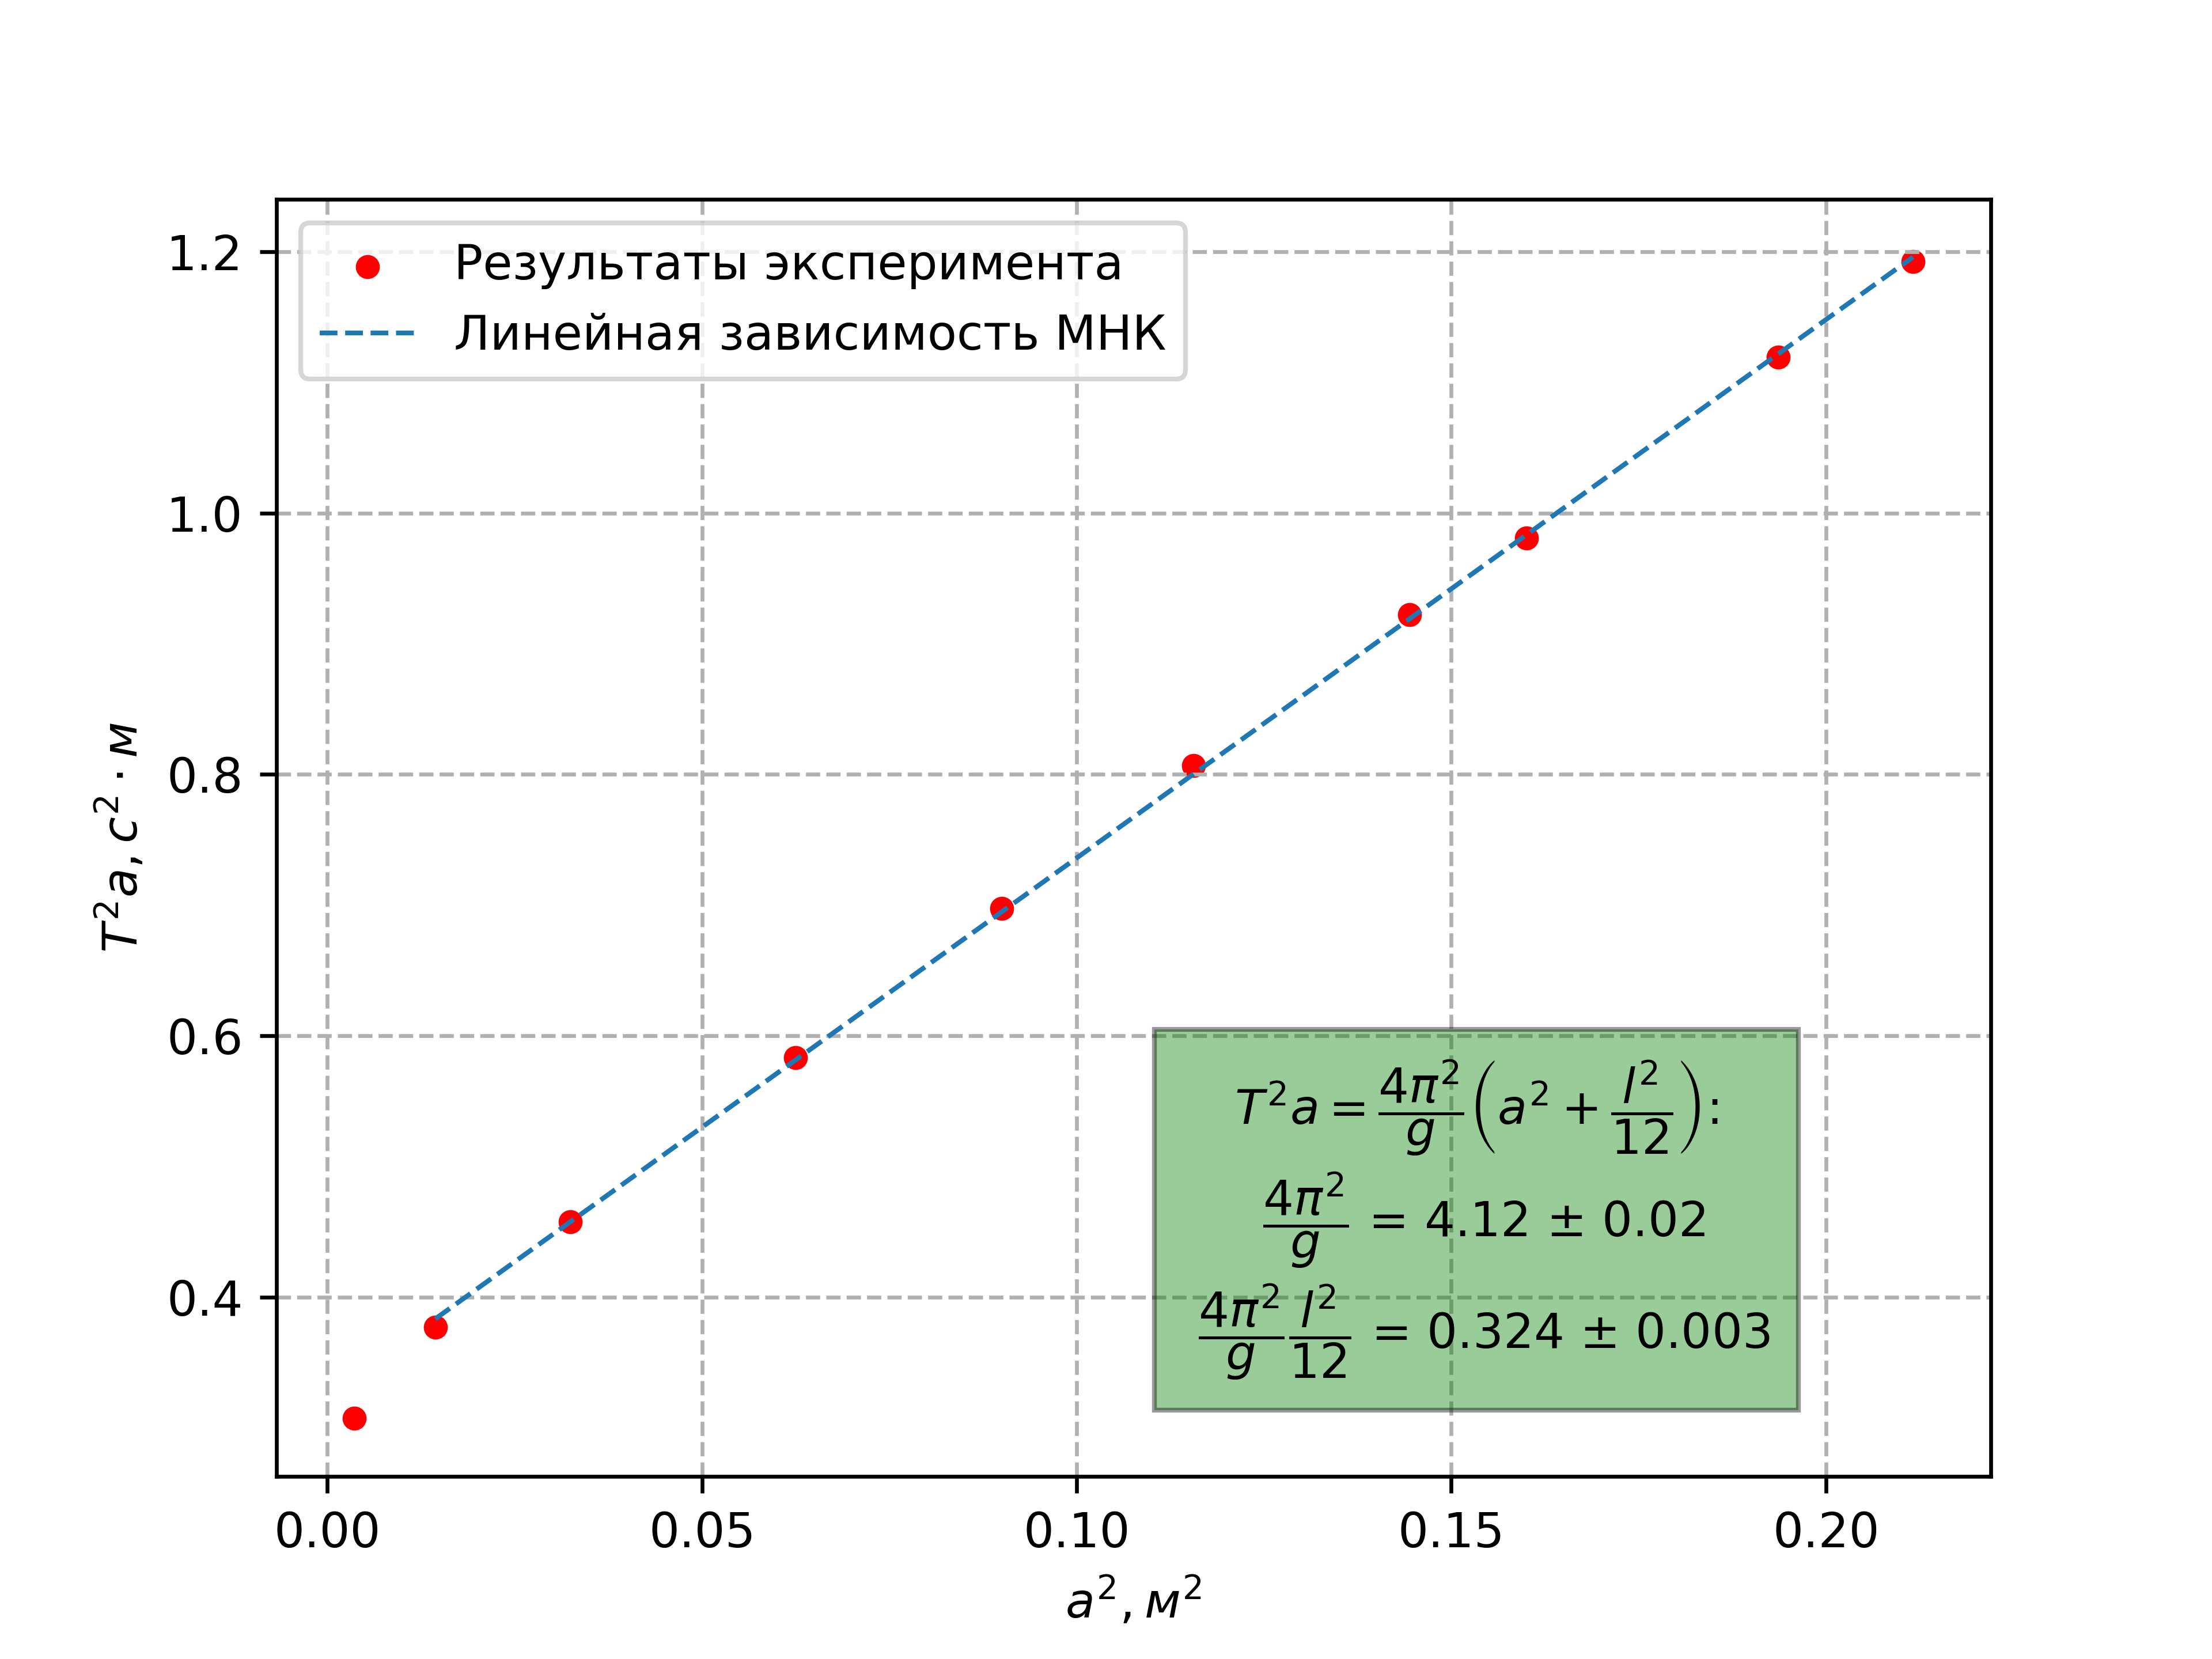
\includegraphics[width=0.75\linewidth]{linear.png}
               	\caption{График $T^2a\left(a^2\right)$}
               	\label{fig:linear}
            \end{figure}

            По методу наименьших квадратов определим коэффициенты $\frac{4\pi^2}{g}$ и $\frac{l^2}{12}$. Погрешности коэффициентов найдём по формулам:
            \begin{multline*}
                k = \frac{4\pi^2}{g} = 4.12: \hspace{0.25cm} \epsilon_k^2 = 4 \cdot \epsilon_T^2 + \epsilon_a^2 \approx 4 \cdot \frac{0.016}{1.5}^2 + \frac{0.0025}{0.1} \Rightarrow \\
                \Rightarrow \epsilon_k \approx 0.033 \Rightarrow \sigma_k = \sqrt{0.02^2 + \left(0.033 \cdot 4.12 \right)^2} \approx 0.14
            \end{multline*}
            
            \begin{multline*}
                b = \frac{4\pi^2}{g} \frac{l^2}{12} = 0.324: \hspace{0.25cm} \epsilon_b^2 = 4 \cdot \epsilon_T^2 + \epsilon_a^2 + \epsilon_k^2 \approx 4 \cdot \frac{0.016}{1.5}^2 + \frac{0.0025}{0.1}^2 + 0.033^2 \Rightarrow \\
                \Rightarrow \epsilon_b \approx 0.047 \Rightarrow \sigma_b = \sqrt{0.003^2 + \left(0.324 \cdot 0.047\right)^2} \approx 0.016
            \end{multline*}

            Находим искомые величины и их погрешности из полученных коэффициентов:
            \begin{align*}
                &g = \frac{4\pi^2}{4.12} \approx 9.58 \text{ м} \cdot \text{с}^{-2} \hspace{0.5cm} \epsilon_g = \epsilon_k \Rightarrow \sigma_g = g \cdot 0.033 = 0.32 \text{ м} \cdot \text{с}^{-2} \\
                &l = \sqrt{12 \cdot 0.324 \cdot \frac{g}{4\pi^2}} \approx 0.97 \text{ м} \hspace{0.5cm} \epsilon_l = \sqrt{\left(\frac{1}{2} \epsilon_g \right)^2 + \left( \frac{1}{2} \epsilon_b \right)} \approx 0.074 \Rightarrow \sigma_l = l \cdot 0.074 = 0.072 \text{ м}
            \end{align*}

        \subsection{Определение приведённой длины}
            Подберём длину математического маятника, у которого период совпадает с периодом физического маятника с $a = 20$ см. При визуальном наблюдении 30 колебаний периоды равны (то есть, принимая погрешность измерения равной 0.03 секунды, получаем, что периоды равны с погрешностью $\sigma = \sqrt{2 \cdot 0.03^2} \approx 0.04$ секунды) при $l \approx 60.5\pm0.2$ см. Приведённая длина, полученная экспериментально, следовательно, равна $60.5\pm0.2$ см. Согласно формуле \ref{eq:length} $l_\text{прив.} = 61.7$ см, что не совпадает в пределах погрешности с экспериментально полученным значением. Для более точного определения приведённой длины следовало сравнивать периоды колебаний мат. и физ. маятников по большему промежутку времени.

        \subsection{Проверка обратимости маятника}
            Проверим обратимость маятника при $a = 20$ см, $l_\text{прив.} = 61.7$ см. Измерим время двадцати колебаний и найдём период: $T_a = 31.52 \div 20 = 1.576 \pm 0.015$ c.

            Теперь точку подвеса разместим на расстоянии $a' = l_\text{прив.} - a = 41.7$ см от центра масс маятника. Период равен $T_{a'} = 31.78 \div 20 = 1.589 \pm 0.015$ с.

			В пределах погрешностей периоды совпадают.

    \pagebreak
    \section{Вывод}
        В ходе работы по косвенным измерениям были найдёны ускорение свободного падения и длина стержня.
        \begin{align*}
            g_\text{экс} &= 9.58 \pm 0.32 \text{ м} \cdot \text{c}^{-2} \hspace{0.5cm} \left(g = 9.81 \text{ м} \cdot \text{c}^{-2}\right)
            \\
            l_\text{экс} &= 0.97 \pm 0.07 \text{ м} \hspace{0.5cm} \left(l = 1\text{м}\right)
        \end{align*}

        Также не вполне успешно была проверна формула для приведённой длины:
        \[
            l_\text{экс} = 60.5 \pm 0.2 \text{ см} \neq l_\text{теор} = 61.7 \text{ см }
        \]
            
        Однако обратимость маятника, при наблюдении которой использовалась теоретическая формула, была доказана точно.
\end{document}